% SC2002 --- Chapter 7: Exception Handling & Generics (0->100 ground-up)
\chapter{Exception Handling \& Generics: Safety at Compile Time and Runtime}
\label{ch:exceptions-generics}

\begin{quote}
\emph{``Errors should be impossible by construction; where they remain possible, they should be impossible to ignore.''} --- Exceptions handle the runtime half; generics handle the compile-time half. Together they make wrong code hard to write and hard to miss.
\end{quote}

\noindent\fbox{\parbox{\dimexpr\linewidth-2\fboxsep-2\fboxrule}{%
\textbf{From zero: built on Ch.~1--5.} We define \emph{error}, \emph{exception}, \emph{throw/catch}, \emph{checked vs.\ unchecked}, and \emph{parametric types} from scratch. No prior generics or exception experience assumed.}}
\vspace{0.4em}

\section*{Learning Outcomes}
After this chapter you will be able to:
\begin{enumerate}[label=(L\arabic*)]
    \item distinguish errors, checked/unchecked exceptions, and when to use each;
    \item write robust try--catch--finally and try-with-resources with correct exception chaining;
    \item design exception hierarchies and apply fail-fast with meaningful messages;
    \item declare and use generic classes/methods, bounded wildcards (PECS), and type erasure consequences;
    \item combine exceptions + generics to build a type-safe, failure-aware API (e.g., \texttt{Result<T>} or \texttt{Repository<T>}).
\end{enumerate}

% ============================================================
\section{Exceptions: Fail Fast, Fail Clearly}
\label{sec:exceptions}
Two bad ways to signal failure: return \texttt{null} (caller forgets to check) and return error codes (easy to ignore, no stack trace). Exceptions make failure \emph{unignorable}: if you do not handle it, the program stops at the call site with a trace.

\begin{figure}[h]
\centering
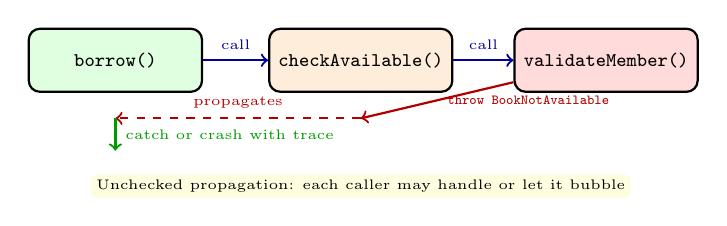
\begin{tikzpicture}[scale=0.82, every node/.style={font=\scriptsize}]
\node[draw,thick,fill=green!12,rounded corners=4pt,minimum width=2.2cm,minimum height=0.8cm] (a) at (0,0) {\texttt{borrow()}};
\node[draw,thick,fill=orange!14,rounded corners=4pt,minimum width=2.2cm,minimum height=0.8cm] (b) at (3.8,0) {\texttt{checkAvailable()}};
\node[draw,thick,fill=red!14,rounded corners=4pt,minimum width=2.2cm,minimum height=0.8cm] (c) at (7.6,0) {\texttt{validateMember()}};
\draw[->,thick,blue!60!black] (a) -- (b) node[midway,above,font=\tiny] {call};
\draw[->,thick,blue!60!black] (b) -- (c) node[midway,above,font=\tiny] {call};
\draw[->,thick,red!70!black] (c) -- (3.8,-0.9) node[midway,right,font=\tiny] {\texttt{throw BookNotAvailable}};
\draw[->,thick,red!70!black,dashed] (3.8,-0.9) -- (0,-0.9) node[midway,above,font=\tiny] {propagates};
\draw[->,thick,green!60!black] (0,-0.9) -- (0,-1.4) node[midway,right,font=\tiny] {catch or crash with trace};
\node[font=\tiny,fill=yellow!12,rounded corners=2pt,inner sep=2pt] at (3.8,-1.95) {Unchecked propagation: each caller may handle or let it bubble};
\end{tikzpicture}
\caption{Exception propagation: a thrown exception unwinds the call stack until caught; uncaught, it terminates with a stack trace.}
\label{fig:exception-propagation}
\end{figure}

\paragraph{Java's hierarchy.} \texttt{Throwable} $\to$ \texttt{Error} (JVM, do not catch) and \texttt{Exception} $\to$ \texttt{RuntimeException} (unchecked) vs.\ other \texttt{Exception} (checked). Checked = compiler forces handling; unchecked = programming errors / recoverable runtime failures.

\begin{center}
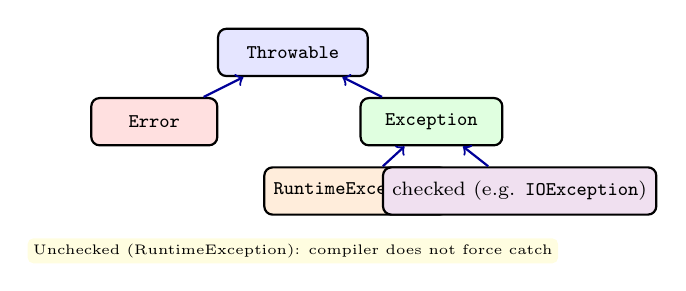
\begin{tikzpicture}[scale=0.80, every node/.style={font=\scriptsize}]
\node[draw,thick,fill=blue!10,rounded corners=3pt,minimum width=1.9cm,minimum height=0.6cm] (t) at (0,1.6) {\texttt{Throwable}};
\node[draw,thick,fill=red!12,rounded corners=3pt,minimum width=1.6cm,minimum height=0.6cm] (e) at (-2.2,0.5) {\texttt{Error}};
\node[draw,thick,fill=green!12,rounded corners=3pt,minimum width=1.8cm,minimum height=0.6cm] (ex) at (2.2,0.5) {\texttt{Exception}};
\node[draw,thick,fill=orange!14,rounded corners=3pt,minimum width=2.2cm,minimum height=0.6cm] (re) at (1.0,-0.6) {\texttt{RuntimeException}};
\node[draw,thick,fill=violet!12,rounded corners=3pt,minimum width=2.0cm,minimum height=0.6cm] (ce) at (3.6,-0.6) {checked (e.g. \texttt{IOException})};
\draw[->,thick,blue!60!black] (e) -- (t);
\draw[->,thick,blue!60!black] (ex) -- (t);
\draw[->,thick,blue!60!black] (re) -- (ex);
\draw[->,thick,blue!60!black] (ce) -- (ex);
\node[font=\tiny,fill=yellow!12,rounded corners=2pt,inner sep=2pt] at (0,-1.55) {Unchecked (RuntimeException): compiler does not force catch};
\end{tikzpicture}
\end{center}

\begin{lstlisting}[language=Java, caption={Checked vs.\ unchecked and try-with-resources with chaining.}]
// Custom checked (recoverable) vs unchecked (programming error)
class BookNotAvailableException extends Exception { // checked: caller must handle
    public BookNotAvailableException(String msg){ super(msg); }
}
class InvalidStateException extends RuntimeException { // unchecked
    public InvalidStateException(String msg){ super(msg); }
}
// try-with-resources: AutoCloseable closed even on exception; addSuppressed preserves cause
void copy(Path src, Path dst) throws IOException {
    try (InputStream in = Files.newInputStream(src);
         OutputStream out = Files.newOutputStream(dst)) {
        in.transferTo(out);
    } catch (IOException e) {
        throw new IOException("copy failed: " + src + " -> " + dst, e); // chain cause
    }
}
\end{lstlisting}

Rules: catch the \emph{most specific} type first; never swallow silently (\texttt{catch(Exception e)\{\}} hides bugs); prefer try-with-resources over manual \texttt{finally} for \texttt{Closeable}s; chain causes with \texttt{new X(msg, cause)} so the root is not lost.

% --- TikZ 2: try-catch-finally flow ---
\begin{figure}[h]
\centering
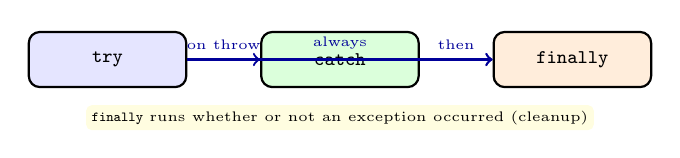
\begin{tikzpicture}[scale=0.82, every node/.style={font=\scriptsize}]
\node[draw,thick,fill=blue!10,rounded corners=4pt,minimum width=2.0cm,minimum height=0.7cm] (try_) at (0,0) {\texttt{try}};
\node[draw,thick,fill=green!14,rounded corners=4pt,minimum width=2.0cm,minimum height=0.7cm] (catch_) at (3.6,0) {\texttt{catch}};
\node[draw,thick,fill=orange!14,rounded corners=4pt,minimum width=2.0cm,minimum height=0.7cm] (fin) at (7.2,0) {\texttt{finally}};
\draw[->,thick,blue!60!black] (try_) -- (catch_) node[midway,above,font=\tiny] {on throw};
\draw[->,thick,blue!60!black] (try_) -- (fin) node[midway,above,font=\tiny] {always};
\draw[->,thick,blue!60!black] (catch_) -- (fin) node[midway,above,font=\tiny] {then};
\node[font=\tiny,align=center,fill=yellow!12,rounded corners=2pt,inner sep=2pt] at (3.6,-0.9) {\texttt{finally} runs whether or not an exception occurred (cleanup)};
\end{tikzpicture}
\caption{Try--catch--finally flow: \texttt{try} for guarded code, \texttt{catch} per exception type, \texttt{finally} for unconditional cleanup.}
\label{fig:try-catch-finally}
\end{figure}

\section{Generics: One Definition, Many Types}
\label{sec:generics}
Without generics, a container holds \texttt{Object} and every retrieval needs a cast (unsafe, verbose). Generics let one class/method work for many types with compile-time checking.

\begin{lstlisting}[language=Java, caption={Generic class and generic method---one definition, type-safe at compile time.}]
// Generic class: Repository works for any T, checked at compile time
class Repository<T> {
    private List<T> items = new ArrayList<>();
    public void add(T t){ items.add(t); }
    public T get(int i){ return items.get(i); } // no cast
}
Repository<Book> books = new Repository<>();
books.add(new Book("Dune")); // ok
// books.add("not a book");  // compile error -- caught early

// Generic method: max works for any Comparable type
<T extends Comparable<T>> T max(T a, T b){ return a.compareTo(b) >= 0 ? a : b; }
\end{lstlisting}

\paragraph{Invariant generics and wildcards.} \texttt{List<Book>} is \emph{not} a subtype of \texttt{List<LibraryItem>} even if \texttt{Book <: LibraryItem} (otherwise you could add an \texttt{AudioBook} to a \texttt{List<Book>}). Wildcards restore flexibility: \texttt{List<? extends LibraryItem>} (producer---read only; PECS: Producer Extends) and \texttt{List<? super Book>} (consumer---write).

% --- TikZ 3: PECS wildcards ---
\begin{figure}[h]
\centering
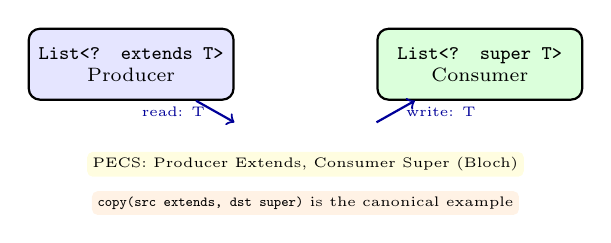
\begin{tikzpicture}[scale=0.82, every node/.style={font=\scriptsize}]
\node[draw,thick,fill=blue!10,rounded corners=4pt,minimum width=2.6cm,minimum height=0.9cm,align=center] (prod) at (0,0) {\texttt{List<? extends T>}\\Producer};
\node[draw,thick,fill=green!14,rounded corners=4pt,minimum width=2.6cm,minimum height=0.9cm,align=center] (cons) at (5.4,0) {\texttt{List<? super T>}\\Consumer};
\draw[->,thick,blue!60!black] (prod) -- (1.6,-0.9) node[midway,left,font=\tiny] {read: T};
\draw[->,thick,blue!60!black] (3.8,-0.9) -- (cons) node[midway,right,font=\tiny] {write: T};
\node[font=\tiny,align=center,fill=yellow!12,rounded corners=2pt,inner sep=2pt] at (2.7,-1.55) {PECS: Producer Extends, Consumer Super (Bloch)};
\node[font=\tiny,align=center,fill=orange!10,rounded corners=2pt,inner sep=2pt] at (2.7,-2.15) {\texttt{copy(src extends, dst super)} is the canonical example};
\end{tikzpicture}
\caption{PECS for wildcards: producers use \texttt{extends} (you read Ts out), consumers use \texttt{super} (you write Ts in).}
\label{fig:pecs}
\end{figure}

\paragraph{Erasure.} Java implements generics by \emph{type erasure}: generic types are checked at compile time then erased to \texttt{Object} (or bounds) at runtime. Consequences: cannot \texttt{new T()}, cannot \texttt{instanceof List<String>}, and primitive types need boxing (\texttt{List<Integer>} not \texttt{List<int>}). Overloads differing only by generic argument erase to the same signature and are illegal.

\section{Putting It Together: A Type-Safe, Failure-Aware API}
\label{sec:putting-together}
Combine exceptions + generics to design an API that is hard to misuse.

\begin{lstlisting}[language=Java, caption={Generic Result<T> captures success/failure without null or error codes.}]
sealed interface Result<T> permits Ok, Err {}
record Ok<T>(T value) implements Result<T> {}
record Err<T>(String message, Throwable cause) implements Result<T> {}

class Library {
    Result<Loan> tryBorrow(String memberId, String bookId){
        try {
            Member m = members.find(memberId);
            Book b = books.find(bookId);
            if (!b.isAvailable()) return new Err<>("book unavailable", null);
            if (!m.canBorrow())   return new Err<>("member limit reached", null);
            Loan ln = Loan.create(m,b);
            return new Ok<>(ln);
        } catch (Exception e){ return new Err<>("borrow failed", e); }
    }
}
\end{lstlisting}

\paragraph{Why this helps.} Callers cannot ignore failure (must handle \texttt{Err}), no \texttt{null} ambiguity, and the success type is generic (\texttt{Result<Loan>} vs.\ \texttt{Result<Book>}) so mixing them is a compile error. For recoverable I/O failures prefer checked exceptions or \texttt{Result}; for programming errors prefer unchecked with fail-fast preconditions (\texttt{Objects.requireNonNull}, \texttt{checkArgument}).

\paragraph{Wildcards in APIs.} Use PECS at API boundaries: \texttt{void addAll(Collection<? extends T> src)}, \texttt{void drainTo(Collection<? super T> dst)}. Inside the implementation, concrete \texttt{T} suffices. This maximises caller flexibility without weakening guarantees.

\begin{remark}[Exceptions vs.\ Result]
Java's idiom is exceptions for exceptional paths and \texttt{Optional<T>}/\texttt{Result<T>} for expected absence/failure. Pick one style per module and be consistent; mixing both for the same failure confuses callers.
\end{remark}

\subsection{Erasure Pitfalls Worked}
\begin{lstlisting}[language=Java, caption={Erasure pitfalls and workarounds.}]
// Cannot overload on generic type alone -- erases to same signature
// void foo(List<String> a) {} void foo(List<Integer> a) {} // compile error

// instanceof with generics -- test via wildcard + cast with warning suppression
boolean isStringList(Object o){
    if (!(o instanceof List<?> l)) return false;
    return !l.isEmpty() && l.get(0) instanceof String;
}
// Creating arrays of generics -- use collections or Array.newInstance with type token
<T> T[] makeArray(Class<T> tok, int n){
    @SuppressWarnings("unchecked") T[] a =
        (T[])java.lang.reflect.Array.newInstance(tok,n);
    return a;
}
\end{lstlisting}
{\sloppy
Bounded type parameters (\texttt{<T extends} \texttt{Comparable<? super T>>}) look noisy but enable \texttt{max} over any comparable hierarchy. Read them as ``T can be compared to itself or a supertype.'' When the bound is complex, introduce a helper interface to name it.\par
}

{\sloppy
\paragraph{Nullability and Optional.} Generics and \texttt{Optional<T>} jointly eliminate many \texttt{null} checks: return \texttt{Optional<Book>} instead of nullable \texttt{Book}, and the compiler forces callers to handle absence. Never use \texttt{Optional} as a field type---it is for return values and stream pipelines.\par
}

\subsection{Testing Generics and Exceptions}
Test generics with at least two instantiations (\texttt{Repository<Book>} and \texttt{Repository<Member>}) to catch raw-type leakage. Test exceptions with \texttt{assertThrows} for the happy-path failure and with a try-with-resources test that the resource is closed even when an exception is thrown (verify via a spy \texttt{Closeable}). For \texttt{Result<T>}, test both \texttt{Ok} and \texttt{Err} branches and that \texttt{Err} preserves the cause chain for debugging.

\section{Chapter Notes}
Checked exceptions are a Java distinctive; many languages use only unchecked (Kotlin, C\#). Bloch (Effective Java) Items 70--77 cover exception design; Item 26--33 cover generics and PECS. Erasure was a compatibility choice (Java 5); C\# reifies generics at runtime.

\section{Exercises}
\label{sec:ch07-exercises}
\begin{enumerate}[label=E7.\arabic*, leftmargin=*, itemsep=0.8em]
    \item \textbf{Checked vs.\ unchecked.} \texttt{BookNotAvailable} on borrow---checked or unchecked? Justify via ``can the caller reasonably recover?'' Give one example of each in the library domain.
    \item \textbf{Swallowed exception.} Find the bug: \texttt{try\{ save(); \} catch(Exception e)\{\}}. Show a failure it hides, then fix with specific catch + chaining + logging.
    \item \textbf{Generics safety.} Without generics, a \texttt{List} holding \texttt{Book} and \texttt{Member} compiles but fails at runtime. Rewrite with \texttt{Repository<T>} and show the compile-time error that now prevents the mix-up.
    \item \textbf{PECS drill.} Write \texttt{copy(List<? extends T> src, List<? super T> dst)}. Explain why \texttt{src} is \texttt{extends} and \texttt{dst} is \texttt{super} and what goes wrong if you swap them.
    \item \textbf{Erasure consequence.} Explain why \texttt{new T()} and \texttt{instanceof List<String>} are illegal after erasure. Propose a workaround for each (factory/type token).
\end{enumerate}
% End of Chapter 7
